\documentclass[a4paper,12pt]{article}
\usepackage{geometry}
\geometry{a4paper, margin=1in}

\usepackage{amsmath, amssymb}

\usepackage{tikz}

\usepackage{graphicx}
\usepackage{caption}

\usepackage{fancyhdr}
\usepackage{graphicx}
\usepackage{titlesec}
\usepackage{titling}
\usepackage{xcolor}
\usepackage{hyperref}
\hypersetup{
    colorlinks=true,
    linkcolor=blue,
    filecolor=magenta,      
    urlcolor=cyan,
}

% Header and Footer
\pagestyle{fancy}
\fancyhf{}
\fancyhead[L]{
\includegraphics[height=0.8cm]{logo.jpg}} % Include your institution logo
\fancyhead[C]{\footnotesize \textbf{\courseName}}
\fancyhead[R]{
\includegraphics[height=0.8cm]{ionq_logo_simple.png}}

\fancyfoot[L]{\projectName}
\fancyfoot[C]{Page \thepage}
\fancyfoot[R]{\today}

% Title formatting
\pretitle{\begin{center}\LARGE \bfseries}
\posttitle{\end{center}\vspace{0.5cm}}
\preauthor{\begin{center}\normalsize}
\postauthor{\end{center}}
\predate{\begin{center}\small}
\postdate{\end{center}\vspace{1cm}}

% Section formatting
\titleformat{\section}[block]{\Large\bfseries}{\thesection}{1em}{}
\titleformat{\subsection}[block]{\large\bfseries}{\thesubsection}{1em}{}
\titleformat{\subsubsection}[block]{\bfseries}{\thesubsubsection}{1em}{}

% Custom commands for student details
%\newcommand{\studentName}{Hyunseong Kim}
%\newcommand{\studentID}{20195048}
\newcommand{\courseName}{2024 IonQ summer Mentoring}
%\newcommand{\courseCode}{MM4020}
\newcommand{\assignmentTitle}{OptTrot}
%\newcommand{\dueDate}{June 30, 2024}

\newcommand{\projectName}{OpTrot}

\newtheorem{theorem}{Theorem}
\newtheorem{lemma}{Lemma}
\newtheorem{definition}{Definition}

\begin{document}

% Title Section
\begin{center}
%    %
\includegraphics[width=0.15\textwidth]{logo.png}\par\vspace{1cm} % Include your institution logo
%    {\scshape \courseName \par}
%    {Final Assignment \par}
%    \vspace{0.5cm}

    \vspace{0.5cm}
    {\Large\bfseries \assignmentTitle \par}
    {\large Optimized Trotterized circuit library \par}
    \vspace{1cm}
    {
    \noindent
    \begin{minipage}{0.45\textwidth}
        \centering
        \textbf{Memebers}

        Hyunseong Kim

        Gaya Yun

        Hanseo Kim
    \end{minipage}
    \begin{minipage}{0.45\textwidth}
        \centering
        \textbf{Mentor}

        Sayomeo Ray
    \end{minipage}
    }
%    {\itshape \studentName \par}
%    {Student ID: \studentID \par}
%    \vspace{0.5cm}
%    {\large \today \par}
    \begin{abstract}
    Abstract
    \end{abstract}
\end{center}


%\tableofcontents
%wpage

\section{Introduction}

Trotterization is a standard method used to implement a time evolution operator 
by combining several local Hamiltonian evolution operators.
In quantum computing, the method has an advantange of preserving the local structure of 
the Hamiltonian on a dynamic circuit \cite{childs_theory_2021}.
However, Trotterization method increases circuit depth with linear order.
If the time evolution was an ultimate goal to achieve in quantum circuit, 
it could be meaningful, but in the most algorithms and applications, time evolution 
is just a part of the whole process. 
In these cases, the increased circuit depth can lead to a loss of precision, making the algorithm less practical.
By the limitation, there are many alternative methods to implement a time evolution operator 
with shorter depth circit than Trotterization, such as 
linear combination of unitary(LCU) method\cite{dewolf2023quantumcomputinglecturenotes}, Qubitization\cite{Low_2019}, 
Taylorization\cite{PhysRevLett.114.090502}, and Fractional query\cite{Berry_2014}.
Such methods make the evolution circuit more practical, however, they loose 
identity of the given system, especially the cases, when the given hamiltonian is nearly commute
or local observable was a dominant feature\cite{childs_theory_2021}. 


\section{Optimizing a circuit with commuting pairs}

\section{Pauli Frame method}

\section{}

\section{Terminology and basic theorems}

Let $S$ be $n$-simplex determined by $n+1$ number of vertices, $\{v_i\}_{i=1}^{n+1}$ in $\mathbb{R}^n$.
\begin{definition}\textbf{Sperner coloring}

    A given simplex $S$ of triangulation $P$ with $V_p$ inner vertices,
    \begin{itemize}
        \item $v \in \partial S$ are all distinct.
        \item $v$ in facet of $S$ are colored one of the corner vertices of the same facet.
        \item $v \in V_p$ vertex could have any color of vertex color in $\partial S$.
    \end{itemize}
\end{definition}

\begin{lemma}\textbf{Sperner's lemma}

    About any Sperner's colored triangulation of the given $n$-simplex $S$,
    (Weak): There is a rainbow $n$-simplex in $P$.
    (Strong): There are odd number of rainbow $n$-simplex in $P$.
\end{lemma}

\textit{Proof} 

$n=1$ case: $n$-simplex be a line segment.
Suppose that the two end colors to be $-1$:blue, and $1$:red. 

\begin{center}
    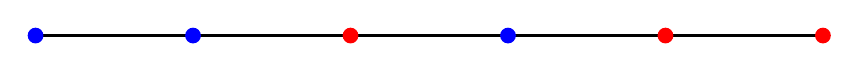
\begin{tikzpicture}
        % Draw the line segment
        \draw[thick] (0,0) -- (10,0);
    
        % Mark the end points
        \fill[blue] (0,0) circle (0.1);
        \fill[red] (10,0) circle (0.1);
        
        % Mark the inner nodes
        \fill[blue] (2,0) circle (0.1);
        \fill[red] (4,0) circle (0.1);
        \fill[blue] (6,0) circle (0.1);
        \fill[red] (8,0) circle (0.1);
    \end{tikzpicture}
\end{center}

If we set a function $f:V \rightarrow \{-1, 1\}$, then 
by the intermediate value theorem, there are odd number of root
so that the odd number of rainbow triangle exist.

$n>1$ case: In the general case, the proof use double counting method.
Let 

\begin{itemize}
    \item $R :=$ \# of rainbow $n$-simplices of $P$.
    \item $Q :=$ \# of $n$-simplices of $P$ having all $[1, \dots n]$ as its color, but $n+1$.
    \item $X :=$ \# of $(n-1)$-simplices of $P$ having all of $[1, \dots, n]$ as its color that contained in $\partial S$
    \item $Y :=$ \# of $(n-1)$-simplices of $P$ having all of $[1, \dots, n]$ as its color that contained in the interior of $S$
\end{itemize}

Each $P$ and $Q$ attached to $\partial S$ has $[1, \dots, n]$ color exactly 
has one $X$. Furthermore, $P$ and $Q$ in interior of $S$, each $Y$ lies between two elements in ($P$,$Q$) or ($Q, Q$).

Thus, the next hold true
\begin{equation}
    R+2Q = X + 2Y
\end{equation}

However, $X$ is odd, since it is $R$ of $n-1$ case, thus $R$ is odd and by the induction it holds for all $n>1$. Done.

\begin{figure}[!ht]
    \centering
    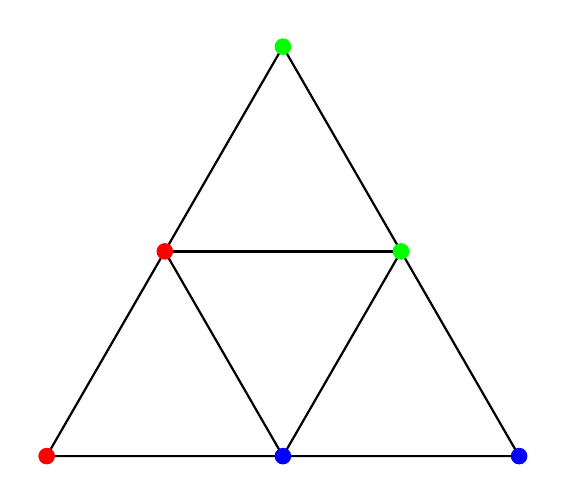
\begin{tikzpicture}
        % Define points
        \coordinate (A) at (0,0);
        \coordinate (B) at (6,0);
        \coordinate (C) at (3,5.2);
        
        % Draw the main triangle
        \draw[thick] (A) -- (B) -- (C) -- cycle;
        
        % Define midpoints
        \coordinate (D) at (3, 0);
        \coordinate (E) at (4.5, 2.6);
        \coordinate (F) at (1.5, 2.6);
        
        % Draw lines connecting midpoints
        \draw[thick] (D) -- (E);
        \draw[thick] (E) -- (F);
        \draw[thick] (F) -- (D);
        
        % Draw vertices with colored circles
        \fill[red] (A) circle (3pt);
        \fill[blue] (B) circle (3pt);
        \fill[green] (C) circle (3pt);
        \fill[blue] (D) circle (3pt);
        \fill[green] (E) circle (3pt);
        \fill[red] (F) circle (3pt);
        
        % Label the vertices
        \node[below left] at (A) {};
        \node[below right] at (B) {};
        \node[above] at (C) {};
        \node[below] at (D) {};
        \node[right] at (E) {};
        \node[left] at (F) {};
        
    \end{tikzpicture}
    \caption{Example of Sperner's lemma in $\mathbb{R}^2$.}
\end{figure}

Huang generalized the lemma with permutation function $N$\cite{Huang2004ONTS},
as 

\begin{definition}
    \label{def:n_permute_function}
    Let $v_i, i \in [k]$ be non-negative integers,
    \begin{equation}
        N(v_1, v_2, \dots, v_k) = \begin{cases}
            1 &  \mbox{It is a permutation and \# of cross is even.}\\
            -1 & \mbox{It is a permutation and  \# of cross is odd.}\\
            0 & \mbox{Not a permuation.}
        \end{cases}
    \end{equation}
\end{definition}

\begin{lemma}\textbf{Generalized Sperner's lemma}
    \label{lemma:gen_sperner}
    Let $C$ be a labeled $k$-chain of $k$-simplices
    of labels $\{0, \dots k \}$. Then,
    \begin{equation}
        N(C) = (-1)^k N( \partial(C))
    \end{equation}
\end{lemma}

If we let $C$ be a triangulized $n$-simplex of Sperner's coloring, 

\section{Roots of complex polynomial}

\subsection{Fundamental theorem of algebra}

\begin{theorem} \textbf{FTA}
    Every polynomial of degree $n$ in $\mathbb{C}$ has exactly $n$ roots on $\mathbb{C}$.
\end{theorem}

To prove FTA, we need two concepts from complex analysis.

\begin{definition}\textbf{Winding Number\cite{Wind_Wolf}}

    Winding number of contour $C$ about point $z_0$ is a positive integer $N(C, z_0)$ that

    \begin{equation}
        N(C, z_0) = \frac{1}{2 \pi i} \oint_C \frac{dz}{z-z_0}
    \end{equation}

    which represents a number that curve pass around a point $z_0$.
\end{definition}

For example, $f(z) = z^n$ about origin $N(f, 0) = n$. 
Using $z = r e^{i \theta}$, $z^n = r^n e^{i n \theta}$.


Cauchy's argument theorem

\begin{theorem} \textbf{Argument theorem\cite{9736615}}
    \label{theorem:Argument}

    For a given meromorphic function, $f$, on complex plane, next identity hold for a given closed contour, $C$

    \begin{equation}
        \frac{1}{2 \pi i} \oint_{C} \frac{f'(z)}{f(z)} dz=  Z - P 
    \end{equation}
    where, $Z$ is a \# of roots inside $C$ and $P$ is a \# of poles in the $C$.
\end{theorem}

If the meromorphic function, $f$, was a finite degree complex polynomial, 
since, every finite degree polynomial has no pole,

\begin{equation}
    \frac{1}{2 \pi i} \oint_{C} \frac{f'(z)}{f(z)} dz=  Z 
\end{equation}


\subsection{Proof of FTA using Sperner's lemma}

Let $p(z) = z^n + a_1 z^{n-1} + \cdots + a_{n-1} z + a_n$ be a monic polynomial
where $a_i \in \mathbb{C}$.

\subsubsection{Existence of n number of rainbow simplex}
For a large enough disk, $D$ whose center is origin of complex plane,
we can make a triangulation of $D$, treating $\mathbb{C}$ as $\mathbb{R}^2$.
Since, $D$ is large near the boundary $p(z) \sim z^n$.
Each vertex is colored by labeling with $\phi(z) = j$ if $z \in R_j, j \in \{0, 1, 2\}$,

\begin{equation}
    \label{eq:phase_color}
    R_j := \{z \in \mathbb{C}\, | \,\frac{2 \pi}{3} j \leq \arg(z) \leq \frac{2 \pi}{3} (j +1)\}
\end{equation}
{
\noindent
\begin{minipage}{0.45\textwidth}
    Now, $z^n$ winds the boundary of $P$ along origin $n$ times.
    Consequently, there exist exactly $n$ number of (0, 1)-simplex on $\partial P$.
    By the definition of $N$, Def (\ref{def:n_permute_function}), only (0, 1)-simplex 
    increases $N$ value, so that

    \begin{equation}
        N(\partial P) = n
    \end{equation}

    By Lemma \ref{lemma:gen_sperner}, $N(P) = n$, consequently there are exactly $n$ number of rainbow simplex 
    in $P$.
\end{minipage}
\hfill
\begin{minipage}{0.45\textwidth}
    \centering
        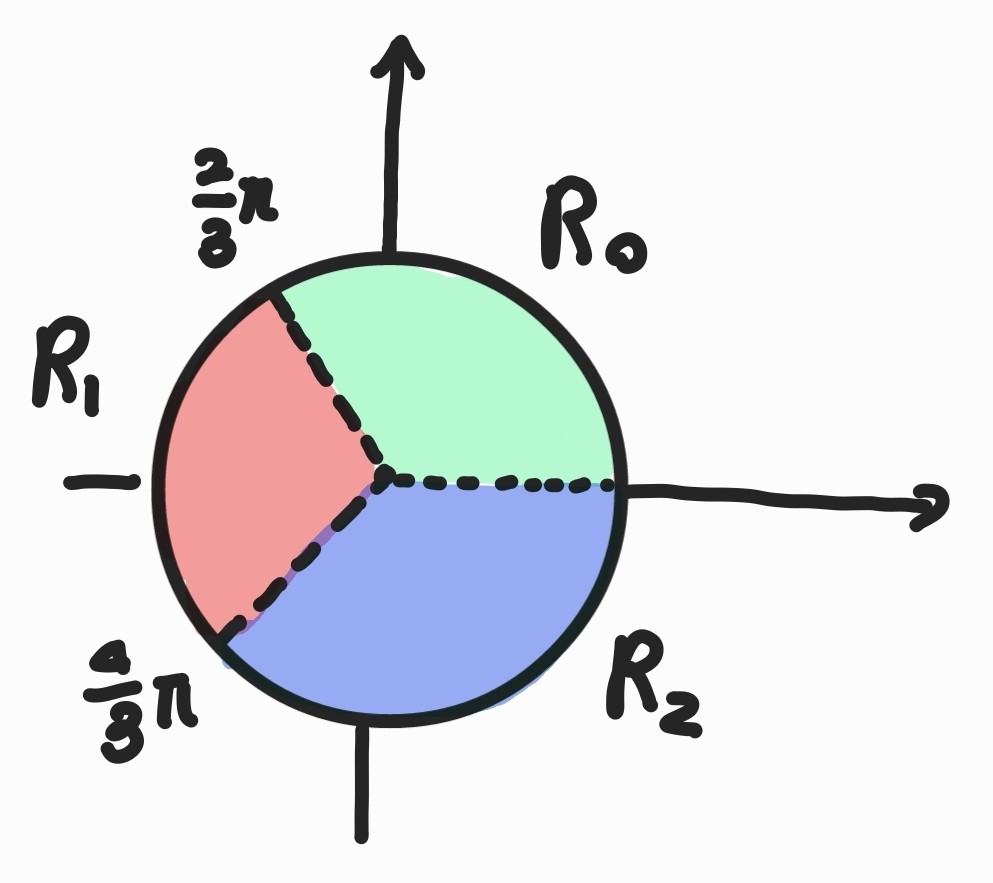
\includegraphics[width=0.8\textwidth]{phase.jpeg}
        \captionof{figure}{Phase of $R_j, j \in \{0, 1, 2\}$}
\end{minipage}
}

\subsubsection{Rainbow simplex to root}
Since, $P$ is fine triangulation of $D$, for the rainbow simplex in interior of $P$ and
their vertex $z_j, z_{j+1}, z_{j+2}$, 
$|p(z_q)- p(z_p)| < \frac{1}{k}, \forall p, q \in {j, j+1, j+2}$, for arbitrary $k>0$.

\vspace{0.5cm}
\textbf{Claim} $|p(z_p)| < \frac{2}{\sqrt{3} k }$ 


\textit{Proof}

WOR, $z_0 \in R_0$ and so do $z_1, z_2$ to be in different $R_i, i \in \{0, 1, 2\}$, 
then since $R_i$ are separated by $\theta = 0, \frac{2 \pi}{3}, \frac{4 \pi}{3}$,
at least, two of three, $z_0, z_1, z_2$ have phase greater or equal than $\pi/3$.
Let such points $z_0$ and $z_1$.
The subspace spanned by $z_1$ with minimizing distance to $z_0$, then the maximum distance
is a $|z_0| \sin(\pi/3)$.

\begin{equation}
    |z_0| \sin(\frac{\pi}{3}) \leq |z_0| |\arg(z_0) - \arg(z_1)| \leq |z_0 - z_1| \frac{1}{k}
\end{equation}

Thus, $|z_0| \leq 2/(\sqrt{3} k)$. 

Polynomial has continuity everywhere, the finer triangulation makes $z_p$ converge to specific point. 
Since, every finite degree polynomial has no pole everywhere, the converged points are all root of the polynomial. 
Done.

\subsection{Root finding}
%----
From the above proof, we found that the proper 3 colors, Eq (\ref{eq:phase_color}),
to be converged to root by finer triangulation.
During the proof, we used arbitrary finite degree polynomial, however,
we can use any complex valued function to find a root.
Since, the convergence only requires 3 colored points and 
triangulation of the domain. 
Any given domain and complex valued function we can 
search roots by the above method in the rainbow simplex to root.

The remained part is how to find a proper triangulation method for the search,
and verify the result whether it is a pole or root.
The verification could be archived by theorem \ref{theorem:Argument}, however,
triangulation methods are various and pros and cons also differ by each method.
The selection of the method requires additional 

Summary the Sperner's based root finding algorithm is

\begin{itemize}
    \item $f$: complex valued function.
    \item $\epsilon >0$: given tolerance. 
\end{itemize}

\begin{enumerate}
    \item Find 3 color points by Eq (\ref{eq:phase_color}).
    \item Make triangulation of the triangle consist of the three points.
    \item Mark the inner vertex by calculating the $f(z)$ and Eq (\ref{eq:phase_color}).
    \item Go to 1 and repeat until the $|f(z_i) - f(z_j)| < \epsilon$ for all vertex of a rainbow triangle.
    \item Verify the cell point using Theorem \ref{theorem:Argument}.
\end{enumerate}

%----

\section{Limitation and further application}

In fact, the above method had been noticed for a long time,
at least before 2005, however, there has been no practical implementation algorithm based on 
Sperner's lemma. 
In 2005, Huang mentioned the practical aspect of the method. 
By him, Sperner's lemma based method requires too much cost
to achieve a desired tolerance error. 
It is not only required for triangulation of the given region,
but also we have to calculate all the function value on the triangulation vertices.

Despite the fact of the inefficient, 
the algorithm does not require 
separated calculation of real and imaginary part calculation.
For example, there was a study about root-finding algorithm
of general complex valued function with given domain by triangulation\cite{10.1145/2699457}.
The method required real and imaginary part of the function separately
to generate the Re(f) =0 and Im(f)=0 line.
The candidate points are overlapped points of the two lines.
Since, Sperner's lemma based algorithm does not have to calculate 
those two zero lines, combine those two method could improve 
root finding routine for general functions.


\section{Conclusion}

In this assignment, we explored how Sperner's lemma can be used to find roots of polynomials on the complex plane. 
This approach shows how combinatorial theories like Sperner's lemma can be applied beyond theoretical studies, 
extending into practical computational algorithms.
Although using Sperner's lemma for root finding in complex polynomials is innovative, 
it is not very practical due to the high computational resources it requires. 
However, this method offers a unique perspective because it doesn't require splitting the function into real and imaginary parts. 
This could potentially simplify some computational processes.

Future studies could look into combining Sperner's lemma with other numerical methods to create more efficient algorithms.
This might help overcome the current limitations and make the lemma more useful for practical applications.


%Bibliography
\bibliographystyle{unsrt}  
\bibliography{references}  

\end{document}
